\documentclass{beamer}


% === PAQUETES === (((
\usepackage[utf8]{inputenc}
\usepackage{amsfonts}
\usepackage{amsmath}
\usepackage{graphicx}
\usepackage{anysize} 
% )))

% === DATOS === (((
% \pdfinfo{%
	% /Title    (Tarea <++> de Ecuaciones Diferenciales)
	% /Author   (Sandra Elizabeth Delgadillo Alemán)
% }
\marginsize{1cm}{1cm}{1cm}{1cm} 
\pagestyle{empty}
% )))

% === TITULO === (((
\newcommand{\titulo}{
	\begin{minipage}{0.25\linewidth}
		\includegraphics[width= 0.9 \linewidth]{IMAGENES/log23.png}
	\end{minipage}
	\begin{minipage}{0.75\linewidth}
		\begin{center}
			\bfseries
			CENTRO DE CIENCIAS BÁSICAS \\
			DEPARTAMENTO DE MATEMÁTICAS Y FÍSICA \\
			ACADEMIA DE MATEMÁTICA AVANZADAS
		\end{center}
	\end{minipage}\\
	\begin{table}[ht]
		\centering
		\begin{tabular}{|*{3}{l|}p{3cm}|}
			\hline
			\textbf{Nombre del Estudiante:} & & \textbf{Fecha:} & \\ \hline
			\textbf{Materia:} & Ecuaciones Diferenciales & \textbf{Carrera:} &  \\ \hline
			\textbf{Profesor:} & Sandra Elizabeth Delgadillo Alemás & \textbf{Semestre:} & \\ \hline
			\textbf{Periodo:} & () Enero--Junio () Agosto--Diciembre & & \\ \hline
			\textbf{Tipo de Examen:} & Parcial: 1() \hspace{2mm} 2() \hspace{2mm} 3() & \textbf{Calificación:} & \\ \hline
		\end{tabular}
	\end{table}
} 
% )))


\begin{document}
\frame{\titlepage}

\section{3. Problemas de Valor Inicial.} % (((

\begin{frame}
	\frametitle{3. Problemas de Valor Inicial.}
	\vspace{-2mm} Cuando modelamos matemáticamente un fenómeno a través de ecuaciones diferenciales, generalmente nos interesa resolver la ecuación diferencial, sujeta a condiciones prescritas sobre la función y sus derivadas, la cuál nos conduce a:
	\begin{block}{Problema de Valor Inicial.}
		Este problema consiste en resolver la E.D. \vspace{-2mm}
		\[
			F \big(\color{blue} x \color{black} \;,\; \color{red} y \color{black} (x) \;,\; \color{green!50!black} y\,' \color{black}(x) , \;\ldots,\; \color{magenta} y^{(n)} \color{black}(x)\big) = 0,  \mbox{ en un intervalo } I,
		\]
		que contiene a \(t_0\), sujeto a las condiciones: \vspace{-2mm}
		\[
			\color{red} y \color{black} (t_0) = y_0 \;,\; \color{green!50!black} y\,' \color{black} (t_0) = y_1 , \;\ldots,\; \color{magenta} y^{(n-1)} \color{black} (t_0) = y_{n-1},
		\]
		donde \(y_0 \;,\; y_1, \;\ldots,\; y_{n-1}\), son constantes reales específicas. \\
		A los valores dados de la función y sus derivadas se les conoce como \textbf{condiciones iniciales}.
	\end{block}
\end{frame}

\subsection{P.V.I. Primer Orden.} % (((

\begin{frame}[c]
	\frametitle{P.V.I. de \(1^{er}\) Orden.}
	\begin{columns}
		\column{0.6\textwidth}
		\begin{definition}
			Se define un \textbf{Problema de Valor Inicial de Primer Orden}, como el sistema,
			\[
				F \big(\color{blue} x \color{black} \;,\;  \color{red} y \color{black} (x) \;,\; \color{green!50!black} y\,' \color{black} (x) \big) =0 \;,\; \hspace{3mm} \color{red} y \color{black} (x_0) = y_0.
			\]
			ó, en forma normal,
			\[
				\color{green!50!black} y\,' \color{black} (x) = f \big(x \;,\; y(x)\big) \;,\; \color{red} y \color{black} (x_0) = y_0.
			\]
		\end{definition}
		\column{0.4\textwidth}
		\begin{tikzpicture}[>=latex, scale=1.2]
			\draw [->] (-2,0) -- (2,0);
			\draw [->] (0,-2.5) -- (0,2.5);
			\clip (-2,-2) rectangle (2,2);
			\draw [thick , blue , rotate=15 , domain=-1:1.5] plot(\x , {pow(0.75*\x-0.3,3) +0.5});
			\draw [black!60,rotate=15 , domain=-1:1.5] plot(\x , {pow(0.75*\x-0.3,3) +1.25});
			\draw [black!60,rotate=15 , domain=-1:1.5] plot(\x , {pow(0.75*\x-0.3,3) -0.6});
			\filldraw [red, dashed] (0,0.9) node [left] {\footnotesize \(y_0\)} --++ (0.9,0) circle (1.5pt) --++ (0,-0.9) node [below] {\footnotesize \(x_0\)};
		\end{tikzpicture}
	\end{columns}
\end{frame}

\begin{frame}[t]
	\frametitle{Ejemplo.}
	\begin{example}
		Sea \(y(x) = ce^{-2x} + e^x\) una familia monoparamétrica de soluciones de la E.D. 
		\[
			y\,' + 2y = 3e^x.
		\]
		Determine la solución del P.V.I. formado pr la E.D. y la C.I. \(y(0) = 1/3\). y esboza su curva integral.
		Luego, determina la curva integral que pasa por \((-1,2)\) y esboza su gráfica.
	\end{example}
	\textbf{Solución.} Debemos determinar el valor de \(c\) en la solución general de tal forma que \(y(0) = -1/3\). \vspace{-4mm}
	\[
		\begin{array}{rrcl}
			&y(0) & = & ce^{-2(0)} +e^0 = - \dfrac{1}{3} \\[3mm]
			\iff &c+1& = & - \dfrac{1}{3} \;\iff\; c= - \dfrac{4}{3}.
		\end{array}
	\]
\end{frame}

\begin{frame}[t]
	\frametitle{Ejemplo.}
	\vspace{-3mm}
	\(\therefore \hspace{5mm} y(x) = - \dfrac{4}{3} e^{-2x} +e^x\) es una solución particular que satisface el P.V.I dado.
	\begin{figure}[ht]
		\centering
		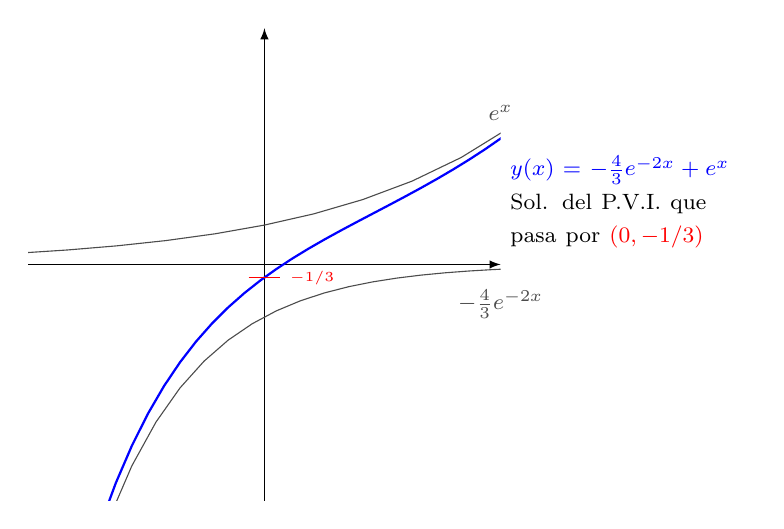
\begin{tikzpicture}[>=latex]
			\draw [->] (-3,0) -- (3,0);
			\draw [->] (0,-3) -- (0,3);
			\node [blue, below right, text width=3cm] at (3,1.5) {\footnotesize \(y(x) = - \frac 43e^{-2x} +e^x\) \color{black} Sol. del P.V.I. que pasa por \color{red} \((0,-1/3)\)};
			\node [black!70, above=2mm] at (3,1.5) {\footnotesize \(e^x\)};
			\node [black!70, below=2mm] at (3,0) {\footnotesize \(- \frac 43e^{-2x}\)};
			\clip (-3,-3) rectangle (3,3);
			\draw [black!70, xscale=2.5, yscale=0.5, domain=-3:3] plot(\x , {exp(\x)});
			\draw [black!70,xscale=2.5, yscale=0.5, domain=-3:3, samples=50] plot(\x , {-1.33*exp(-2*\x)});
			\draw [blue, xscale=2.5, yscale=0.5, thick , domain=-1:3, samples=50] plot(\x , {exp(\x)-1.33*exp(-2*\x)});
			\draw [red] (-0.2,-0.17) --++ (0.4,0) node [right] {\tiny \(-1/3\)};
		\end{tikzpicture}
	\end{figure}
\end{frame}

\begin{frame}[t]
	\frametitle{Ejemplo.}
	\vspace{-4mm}
	Debemos ver el valor de \(c\) en la solución general, de tal forma que \(y(-1) = 2\). \vspace{-4mm}
	\[
		\begin{array}{rrcl}
			&y(-1) &=& ce^{-2(-1)} +e ^{-1} = 2 \\
			\iff & ce^2 + \dfrac{1}{e} &=& 2 \\
			\iff &c&=& \dfrac{2}{e^2} - \dfrac{1}{e^3} = \dfrac{2e-1}{e^3} = \dfrac{2-e^{-1}}{e^2} \approx 0.22
		\end{array}
	\]
	\(\therefore \; y(x) = \dfrac{2e-1}{e^3} e^{-2x} +e^x\) es una sol. particular que satisface el P.V.I.
	\begin{figure}[ht]
		\centering
		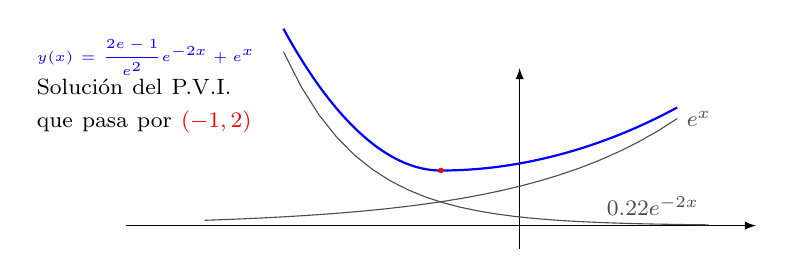
\begin{tikzpicture}[>=latex]
			\draw [->] (-5,0) -- (3,0);
			\draw [->] (0,-0.3) -- (0,2);
			\draw [black!70, yscale=0.5, xscale=2,  domain=-2:1] plot(\x , {exp(\x)}) node [right] {\footnotesize \(e^x\)};
			\draw [black!70, yscale=0.5, xscale=2,  domain=-1.5:1.2] plot(\x , {0.22*exp(-2*\x)}) node [above left] {\footnotesize \(0.22e^{-2x}\)};
			% \draw [blue , thick , yscale=0.5, xscale=2, domain=-1.4,1] plot(\x , {0.22*exp(-2*x) +exp(\x)});
			\draw [thick , blue] (-3,2.5) node [below left, text width=3cm] {\tiny \(y(x) = \dfrac{2e-1}{e^2} e^{-2x} +e^x \) \footnotesize \color{black}Solución del P.V.I. que pasa por \color{red} \((-1,2)\)} parabola bend (-1,0.7) (2,1.5);
			\fill [red] (-1,0.7) circle (1pt);
		\end{tikzpicture}
	\end{figure}
\end{frame}

\begin{frame}[t]
	\frametitle{Ejemplo.}
	\begin{example}
		Resuelve el P.V.I. dado por \(y\,' = -\dfrac{y}{x}\), \(y(2) =-3\), \(y \ne 0\), y esboza su gráfica de su curva solución.
	\end{example}
	\textbf{Solución.} Sabemos que la solución general de la E.D. es \(x^2+y^2=c\).\\
	Observamos que la ec. es equivalente a \(x^2+y(x) ^2=c\).\\
	Debemos determinar el valor de \(c\) en la sol. gral. de tal forma que \(y(2) = -3\).	Evaluamos en \(x=2\)
	\[
		\begin{array}{rrcl}
			& (2) ^2+y(2) ^2& = &c \\[2mm]
			\iff & (2) ^2+(-3) ^2& = &c \\[2mm]
			\iff & c& = &13.
		\end{array}
	\]
\end{frame}

\begin{frame}[t]
	\frametitle{Ejemplo.}
	\begin{columns}
		\column{0.5\textwidth}
		\(\therefore \hspace{5mm}\) La solución implícita que satisface la condición inicial es
		\[
			x^2+y^2=13
		\]
		y la solución particular explícita que satisface la C.I. \(y(2) =-3\) es
		\[
			y(x) = - \sqrt{13-x^2}.
		\]
		\column{0.5\textwidth}
		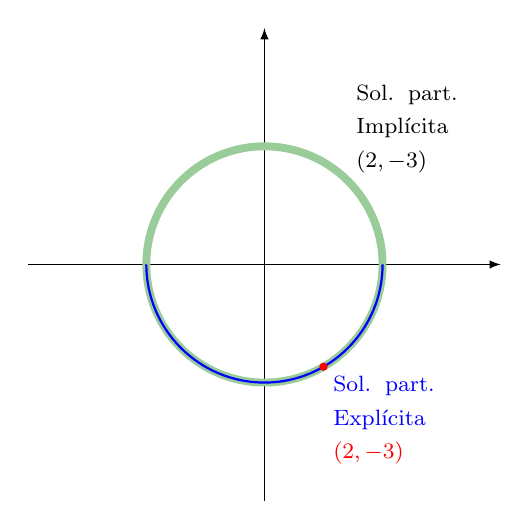
\begin{tikzpicture}[>=latex, scale=1.5]
			\draw [->] (-2,0) -- (2,0);
			\draw [->] (0,-2) -- (0,2);
			\draw [line width=1mm, green!50!black!40] (0,0) circle (1cm) node [above right=1cm, text width=1.5cm] {\footnotesize \color{black} Sol. part. Implícita \((2,-3)\)};
			\draw [thick , blue ] (-1,0) arc (180:360: 1 cm);
			\fill [red] ({cos(60)} , {sin(-60)}) circle (1pt) node [below right, text width=1.5cm] {\footnotesize \color{blue} Sol. part. Explícita \color{red} \((2,-3)\)};
		\end{tikzpicture}
	\end{columns}
\end{frame}

\begin{frame}[t]
	\frametitle{Ejercicio.}
	\vspace{-5mm}
	\begin{alertblock}{Ejercicio.}
		Sea \(xy=3(y-1) +ce^{-y}\) la sol. gral de la E.D. 
		\[
			y+(xy+x-3y) y\,' =0.
		\]
		Determina la solución imlpícita y explícita (si es posible) que satisface la condición inicial \(y(2) = 1/3\).
	\end{alertblock}
	\textbf{Solución.} Sustituimos \(x=2\) y \(y=1/3\) en la solución general \(xy=3(y-1) ce^{-y}\), para determinar el valor de \(c\).
	\[
		\begin{array}{rcl}
			(2) (1/3) & = & 3 (1/3 -1) +ce^{-1/3} \\[2mm]
			2/3 & = & -2+ce^{-1/3} \\[2mm]
			8 & = & ce^{-1/3} \\[2mm]
			c & = & 8e^{1/3} /3 \approx 3.72
		\end{array}
	\]
\end{frame}

\begin{frame}[t]
	\frametitle{Ejercicio.}
	\vspace{-4mm}
	\(\therefore \hspace{3mm}\) la solución particular implícita que cumple con la condición inicial dada es \(xy=3(y-1) + \dfrac{8e^{1/3}}{3} e^{-y}\). Gráficamente
	\begin{columns}
		\column{0.7\textwidth}
		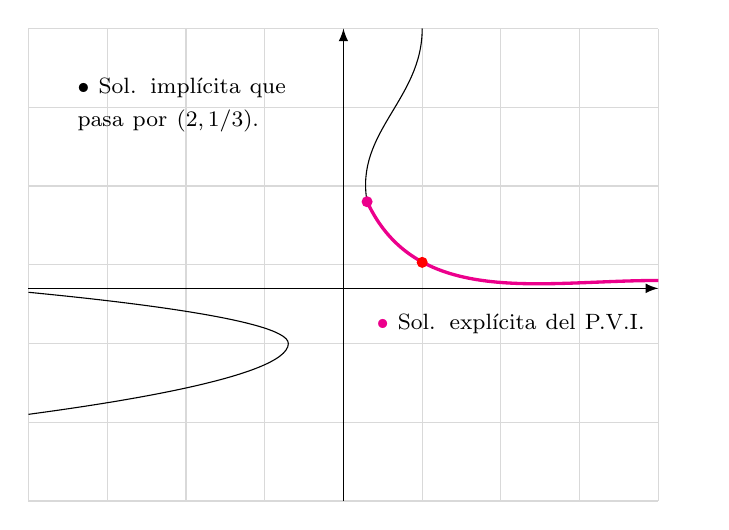
\begin{tikzpicture}[>=latex]
			\draw [gray!30] (-4,-3) grid (4,3);
			\draw [semithick ,->] (-4,-0.3) -- (4,-0.3);
			\draw [semithick ,->] (0,-3) -- (0,3);
			\draw (1,3) to [out=-90 , in=100] (0.3,0.8);
			\draw [very thick ,magenta] (0.3,0.8) to [out=-65, in=180] (4,-0.2); 
			\fill [magenta] (0.3,0.8) circle (2pt);
			\draw [rotate=90] (-1.9,4) parabola bend (-1,0.7) (-0.35,4);
			\fill [red] (1,0.03) circle (2pt);
			\node [below right, text width=3cm] at (-3.5,2.5) {\footnotesize \(\bullet\) Sol. implícita que pasa por \((2,1/3)\).};
			\node [below right, text width=4cm] at (0.3,-0.5) {\footnotesize \color{magenta} \(\bullet\) \color{black} Sol. explícita del P.V.I.};
		\end{tikzpicture}
		\column{0.3\textwidth}
		No es posible determinar de manera algebraica la solición explícita que pasa por \color{red} \((2,1/3)\).
	\end{columns}
\end{frame}

\begin{frame}[t]
Observamos que existen E.D. que pueden tener una única solución que satisface una condición inicial dada, o puede tener un número infinito de soluciones, o no puede existir ninguna solución. 
	\begin{example}{Por ejemplo.}
		Sea \(y(x) = kx\)  la solución general de la E.D. \(\dfrac{dy}{dx} = \dfrac{y}{x}\). 
		\begin{enumerate}
			\item \textit{Determine la solución que satisface la C.I. \(y(0) = 1\).} \label{e2} \\[2mm]
				\textbf{Solución.} \(y(0) = k(0) = 1 \iff 0=1 !!!\) \\[2mm]
				\hspace{7mm} \(\therefore \hspace{5mm}\) No existe \(k\) tal que \(y(0) =1\). \\[2mm]
				\hspace{7mm} \(\therefore \hspace{5mm}\) No existe solución que pase por \((0,1)\).
			\item \textit{Determine la solución que satisface \(y(1) =1\).} \label{identidad} \\[2mm]
				\textbf{Solución.} \\[2mm]
				Encontremos \(k \in \mathbb{R}\) para \(y(x) = kx\) tal que \(y(1) =1\).
		\end{enumerate}
	\end{example}
\end{frame}

\begin{frame}[t]
	\begin{exampleblock}{}
		\[
			\begin{array}{rcl}
				y(1) & = & k(1) = 1 \\[2mm]
				\therefore \hspace{5mm} k & = & 1
			\end{array}
		\]
		Por lo tanto \(y(x) = x\) es la solución única que pasa por \((1,1)\).
		\begin{enumerate}
			\setcounter{enumi}{2}
			\item \textit{Determine la solución que satisface \(y(0) =0\).} \label{origen} \\[2mm]
				\textbf{Solución.} Encontremos \(k \in \mathbb{R}\), para \(y(x) =kx\) tal que \(y(0) =0\). \vspace{-2mm}
				\[
					\begin{array}{rcl}
						y(0) = k(0) & = & 0 \\[2mm]
						\iff 0 & = & 0
					\end{array}
				\]
				\(\therefore \hspace{5mm} y(x) =kx \;,\; k \in \mathbb{R}\), satisface la condición inicial dada.
				\newcommand{\ejes}{
					\draw [->] (-1,0) -- (1,0);
					\draw [->] (0,-1) -- (0,1);
				} 
				\begin{figure}[ht]
					\centering
					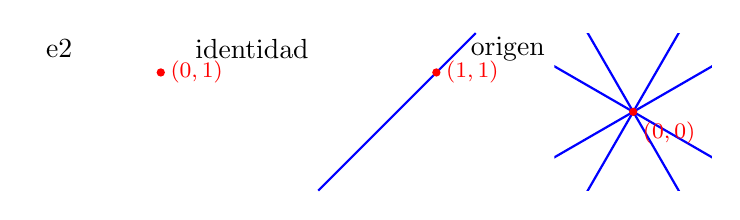
\begin{tikzpicture}[>=latex]
						\ejes 
						\fill [red] (0,0.5) circle (1.5pt) node [right] {\footnotesize \((0,1)\)};
						\node [left] at (-1,0.8) {~\Myref{e2}};
						\begin{scope}[xshift=3cm]
							\ejes
							\draw [blue , thick] (-1,-1) -- (1,1);
							\fill [red] (0.5,0.5) circle (1.5pt) node [right] {\footnotesize \((1,1)\)};
							\node [left] at (-1,0.8) {~\Myref{identidad}};
						\end{scope}
						\begin{scope}[xshift=6cm]
							\ejes
							\node [left] at (-1,0.8) {~\Myref{origen}};
							\clip (-1,-1) rectangle (1,1);
							\draw [rotate=-15,blue , thick] (-1,-1) -- (1,1);
							\draw [rotate=15,blue , thick] (-1,-1) -- (1,1);
							\draw [rotate=-15,blue , thick] (-1,1) -- (1,-1);
							\draw [rotate=15,blue , thick] (-1,1) -- (1,-1);
							\fill [red] (0,0) circle (1.5pt) node [below right] {\footnotesize \((0,0)\)};
						\end{scope}
					\end{tikzpicture}
				\end{figure}
		\end{enumerate}
	\end{exampleblock}
\end{frame}

% )))

% )))

\section{4. Teorema de Existencia y Unicidad (P.V.I. de \(1^{er}\) Orden).} % (((

\begin{frame}[t]
	\frametitle{4. Teorema de Existencia y Unicidad (P.V.I. de \(1^{er}\) Orden).}
	% \begin{alertblock}{Teorema.}
	% \end{alertblock}
	\vspace{-5mm}
	\begin{theorem}
		Dado el P.V.I. \(\dfrac{d y}{dx} = f(x,y)\) con \(y(x_0) = y_0\). Suponga qe \(f\) y \(\dfrac{df}{dy}\) son continuas en un rectángulo \(R\) definido por
		\[
			R = \{(x,y) \;|\; a<x <b \;,\; c<y<d \}, \hspace{5mm} \mbox{que contiene a } (x_0,y_0).
		\]
		Entonces el \alert{P.V.I. tiene solución y es única}, \(\varphi (x)\) en el intervalo \(I_0\) definido por \(x_0-h<x<x_0+h\) con \(h>0\) y además \(I_0 \subseteq (a,b)\).
		\vspace{-2mm}
		\begin{figure}[ht]
			\centering
			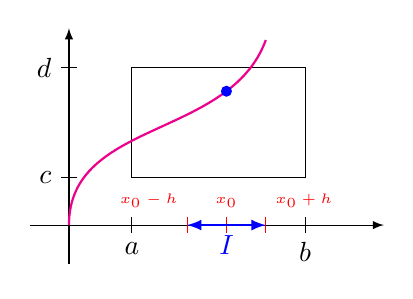
\begin{tikzpicture}[>=latex]
				\draw [->] (-0.5,0) -- (4,0);
				\draw [->] (0,-0.5) -- (0,2.5);
				\draw (0.8,0.6) rectangle (3,2);
				\draw (0.1,0.6) --++ (-0.2,0) node [left] {\(c\)};
				\draw (0.1,2) --++ (-0.2,0) node [left] {\(d\)};
				\draw (0.8,0.1) --++ (0,-0.2) node [below] {\(a\)};
				\draw (3,0.1) --++ (0,-0.2) node [below] {\(b\)};
				\def\radio{0.5}
				\draw [red] (2,-0.1) --++ (0,0.2) node [above] {\tiny \(x_0\)};
				\draw [red] (2-\radio,-0.1) --++ (0,0.2) node [above left] {\tiny \(x_0-h\)};
				\draw [red] (2+\radio,-0.1) --++ (0,0.2) node [above right] {\tiny \(x_0+h\)};
				\draw [thick , blue , <->] (2-\radio,0) to node[below] {\(I\)} (2+\radio,0);
				\draw [thick , magenta] (0,0) to [out=90 , in=250] (2.5,2.35); 
				\fill [blue] (2,1.7) circle (2pt);
			\end{tikzpicture}
		\end{figure}
	\end{theorem}
\end{frame}

\begin{frame}[t]
	\vspace{-3mm}
	\begin{block}{\vspace*{-3ex}}
		\begin{enumerate}
			\item La continuidad de \(f\) nos asegura la existencia de la solución del P.V.I.
			\item La continuidad de \(\dfrac{df}{dy}\) nos da la unicidad de la solución del P.V.I.
		\end{enumerate}
	\end{block}
	\begin{example}
		Considere la E.D. \(\dfrac{dy}{dx} = \dfrac{y}{x}\), \(x \ne 0\), con la condición inicial\\[1mm]
		\begin{minipage}{0.3\linewidth}
			\begin{enumerate}
				\item \(y(0) =1\).
			\end{enumerate}
		\end{minipage}\hspace{5mm}
		\begin{minipage}{0.3\linewidth}
			\begin{enumerate}
				\setcounter{enumi}{1}
				\item \(y(1) =1\).
			\end{enumerate}
		\end{minipage}
		\begin{minipage}{0.3\linewidth}
			\begin{enumerate}
				\setcounter{enumi}{2}
				\item \(y(0) =0\).
			\end{enumerate}
		\end{minipage} \\[2mm]
		Veamos que nos dice el \textsc{T. E. y U.} acerca de la solución del P.V.I. \\
		\textbf{Solución.} La E.D. en su forma normal es: \vspace{-3mm}
		\[
			\dfrac{dy}{dx} = \underbrace{\dfrac{y}{x}}_{f(x,y)}. \hspace{5mm} \begin{array}{c}
				\mbox{Decimos que } f(x,y) = \dfrac{y}{x}.\\[1mm]
				D_f = \mathbb{R} ^2 \setminus \{(x,y) \;|\; x=0\}.
			\end{array}
		\]
	\end{example}
\end{frame}

\begin{frame}[t]
	\begin{exampleblock}{}
		Además \(\dfrac{df}{dy} = \dfrac{1}{x}\), con \(D_{\frac{df}{dy}} = \mathbb{R} \setminus \{(x,y) \;|\; x =0\} \). \\[2mm]
		\begin{columns}
			\column{0.35\textwidth}
			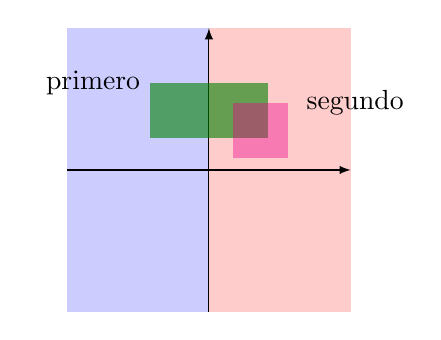
\begin{tikzpicture}[>=latex]
				\draw [white] (-2,0) -- (-1.8,0);
				\fill [red!20] (0,-1.8) rectangle (1.8,1.8);
				\fill [blue!20] (0,-1.8) rectangle (-1.8,1.8);
				\draw [->] (-1.8,0) -- (1.8,0);
				\draw [->] (0,-1.8) -- (0,1.8);
				\fill [green!50!black , opacity=0.6] (-0.75,0.4) rectangle ++(1.5,0.7);
				\fill [magenta, opacity=0.4] (0.3,0.15) rectangle ++(0.7,0.7);
				\node [left] at (-0.75,1.1) {~\Myref{primero}};
				\node [right] at (1,0.85) {~\Myref{segundo}};
			\end{tikzpicture}
			\column{0.65\textwidth}
			Se tienen las siguientes regiones de continuidad
			\[
				\begin{array}{rcll}
					\color{blue} R_1 & = & \{(x,y) \;|& - \infty <x < 0 \;,\; \\[2mm]
					&&&- \infty < y < \infty\} \\[2mm]
					\color{red} R_2 & = & \{(x,y) \;|& 0 <x < \infty \;,\; \\[2mm]
					&&&-\infty < y < \infty\}
				\end{array}
			\]
		\end{columns}
		\begin{enumerate}
			\item \(y(0) =1 \;\implies\; (0,1) \in \mbox{Im} y\). \label{primero} \\[2mm]
				No es posible construir un rectángulo que contenga a \((0,1)\) en donde, tanto \(f\), como \(\dfrac{df}{dy}\) sean continuas.
		\end{enumerate}
	\end{exampleblock}
\end{frame}

\begin{frame}[t]
	\begin{exampleblock}{}
		\begin{enumerate}
				\setcounter{enumi}{1}
			\item \(y(1) =1 \;\implies\; (1,1) \in \mbox{Im} y\). \label{segundo} \\[2mm]
				En este caso, sí es posible construir un rectángulo qu contenga a \((1,1)\) donde tanto \(f \;,\; \dfrac{df}{dy}\) son continuas. \\[2mm]
				\(\therefore \hspace{3mm}\) por el \textsc{T. E. y U.}, existe \(\dfrac{dy}{dx}\) y es única, la sol. que pasa por \((1,1)\) en un intervalo \(I_0 \subseteq (a,b)\).
			\item \(y(0) =0 \;\implies\; (0,0) \in \mbox{Im} y\). \\[2mm]
				No es posible construir un rectángulo cerrado que contenga a \((0,0)\) en el cuál \(f \;,\; \dfrac{df}{dy}\) sean continuas. \\[2mm]
				\(\therefore \hspace{5mm}\) \textsc{T. E. y U.} no es posible aplicarlo.
		\end{enumerate}
	\end{exampleblock}
\end{frame}

% )))

\section{5. Campos Direccionales y Métodos de las Isoclinas.} % (((

\subsection{--- Interpretación Geométrica de la E.D. ---} % (((

\begin{frame}[t]
	\frametitle{5. Campos Direccionales y Métodos de las Isoclinas.}
	\vspace{-5.5mm}
	\begin{columns}
		\column{0.4\textwidth}
		\begin{block}{Forma Analítica}
			\(
				\begin{array}{rcl}
					y\,' & = & f(x,y) \\
					y & = & y(x)
				\end{array}
			\)
		\end{block}
		\column{0.6\textwidth}
		\begin{block}{Geométricamente}
			Campo de direccines o pendientes. \\[2mm]
			Curva Integral.
		\end{block}
	\end{columns}
	\vspace{-2mm}
	\begin{example}
		Considere la E.D. \(\dfrac{dy}{dx} =xy^2\), esboce el campo de pendientes y algunas curvas solución o integrales.
		\vspace{-2mm}
\begin{columns}
    \begin{column}{.4\textwidth}
			\small 
			\begin{tabular}{l|l}
				Puntos & Pendientes \\ \hline
				\(\color{orange} (1,1)\)  & \(dy/dx = (1) (1) ^2=1\) \\
				\(\color{blue} (1,-2)\) & \(dy/dx = (1) (-2) ^2=4\) \\ 
				\(\color{red} (-1,1)\) & \(dy/dx = (-1) (1) =-1\) \\ 
				\(\color{magenta} (0,0)\)  & \(dy/dx = (0) (0) =0\) \\ 
				\(\color{green!50!black} (-1,-2)\)& \(dy/dx =(-1) (-2) ^2=-4\) \\ 
				\((1,2)\)  & \(dy/dx = (1) (2) ^2=4\) \\ 
			\end{tabular}
    \end{column}
    \begin{column}{.5\textwidth}
			\hspace{9mm}
			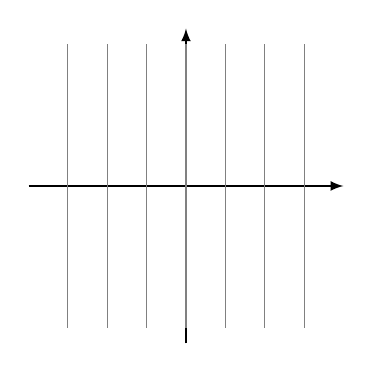
\begin{tikzpicture}[>=latex]
				\draw [semithick,->] (-2,0) -- (2,0);
				\draw [semithick,->] (0,-2) -- (0,2);
				\foreach \n in {-1.5,-1,...,1.5} \draw [gray, thin] (\n,-1.8) --++ (0,3.6);
				\vectorcito{magenta}{0,0}{0}
				\vectorcito{orange}{1,1}{1}
				\vectorcito{blue}{1,-2}{4}
				\vectorcito{red}{-1,1}{-1}
				\vectorcito{green!50!black}{-1,-2}{-2}
				\vectorcito{black}{1,2}{2}
			\end{tikzpicture}
    \end{column}
\end{columns}
	\end{example}
\end{frame}

\begin{frame}[t]
	\begin{example}
		Considere el campo direccional hecho por computadora de la E.D. \(\dfrac{dy}{dx} = \sin x \cos y\) y trace a mano las gráfias de las curvas solución que satisfacen las sig. condiciones iniciales. \vspace{-5mm}
		\begin{columns}
			\column{0.3\textwidth}
		\begin{enumerate}\setlength{\itemsep}{7mm}
				\item \(y(1) =-1/2\). \label{condicion_primera}
				\item \(y(0) = \pi /2\). \label{condicion_segunda}
				\item \(y(-1) =3\). \label{condicion_tercera}
				\item \(y(\pi) =-2\). \label{condicion_cuarta}
			\end{enumerate}
			\column{0.7\textwidth}
				\begin{tikzpicture}[>=latex,scale=0.6]
					\node at (0,0) {\includegraphics[scale=0.6]{FIGURA/xelatex.pdf}};
					\draw [magenta, domain=-3.6:3.6, thick] plot(\x , {-0.5-0.8*cos(1.5*\x r)});
					\draw [magenta, domain=-3.6:3.6, thick] plot(\x , {-2+0.1*cos(1.5*\x r)});
					\draw [magenta, thick] (-3.6,pi/2) -- (3.6,pi/2);
					\draw [magenta, domain=-3.6:3.6, thick] plot(\x , {2.8+0.5*cos(1.5*\x r)});
					\node at (1,-0.5) {~\Myref{condicion_primera}};
					\node at (0,pi/2) {~\Myref{condicion_segunda}};
					\node at (-1,3) {~\Myref{condicion_tercera}};
					\node at (pi,-2) {~\Myref{condicion_cuarta}};
				\end{tikzpicture}
		\end{columns}
	\end{example}
\end{frame}

\begin{frame}[t]
	\begin{exampleblock}{}
		Notamos que \alert{\(\dfrac{dy}{dx} = \sin x \cos y =0\)} implica que \vspace{-5mm}
		\[
			\begin{array}{rcl}
				\sin x=0 & \mbox{o} & \cos y=0 \\[2mm]
				x= k \pi \;,\; k \in \mathbb{Z} & \mbox{o} & y=k \pi + \dfrac{\pi}{2} \;,\; k \in \mathbb{Z} .
			\end{array}
		\]
	\end{exampleblock}
\end{frame}

% )))

\subsection{--- Método de las Isoclinas (igualación) ---} % (((

\begin{frame}[t]
	\frametitle{Método de las Isoclinas (igualación)}
	\begin{definition}
		Una \textbf{isoclina} para una E.D. es un conjunto de puntos \((x,y)\) del plano donde la ecuación diferencial \(y\,' = f(x,y) =c\). Es decir, que las isoclinas son las curvas de nivel de \(f\), es decir \alert{\(f(x,y) =c\).} 
	\end{definition}
	\begin{example}
		Considere la E.D. \(y\,' = 1+x-y\). Obtenga el campo direccional de la E.D. usando el método de las isoclinas.
		\begin{enumerate}
			\item Bosquea la solución que satisface la C.I. \(y(2) =1\) y la sol. que pasa por \((-1,2)\).
			\item ¿Qué se puede decir acerca de las soluciones del inciso anterior cuando \(x \longrightarrow \infty\) o \(x \longrightarrow - \infty\)?.
		\end{enumerate}
	\end{example}
\end{frame}

\begin{frame}[t]
	\begin{exampleblock}{}
		\textbf{Solución.}
		\begin{enumerate}
			\item Isoclinas \(y\,' =1+x-y=c \iff y=1+x-c\).
		\begin{columns}
			\column{0.5\textwidth}
			\small
			\begin{tabular}{r|l}
				\(c\) & Isoclina \\ \hline 
				\(-2\) & \(y_{-2} =1+x+2=x+3\) \\
				\(-1\) & \(y_{-1} =1+x+1=x+2\) \\
				\(-0\) & \(y_{-1} =1+x+0=x+1\) \\
				\(1\) & \(y_{-1} =1+x-1=x\) \\
				\(1\) & \(y_{-1} =1+x-2=x-1\) \\
			\end{tabular}
			\column{0.5\textwidth}
			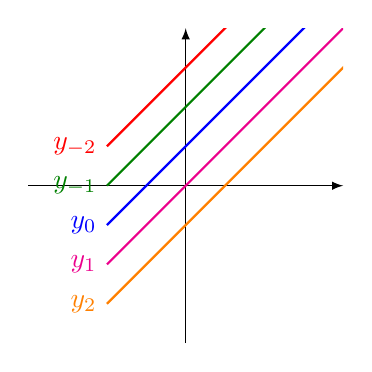
\begin{tikzpicture}[>=latex, scale=0.5]
				\draw [->] (-4,0) -- (4,0);
				\draw [->] (0,-4) -- (0,4);
				\clip (-4,-4) rectangle (4,4);
				\draw [thick , red] (-2,1) node [left] {\(y_{-2}\)} --++ (8,8);
				\draw [thick , green!50!black] (-2,0) node [left] {\(y_{-1}\)} --++ (8,8);
				\draw [thick , blue] (-2,-1) node [left] {\(y_0\)} --++ (8,8);
				\draw [thick , magenta] (-2,-2) node [left] {\(y_1\)} --++ (8,8);
				\draw [thick , orange] (-2,-3) node [left] {\(y_2\)} --++ (8,8);
			\end{tikzpicture}
		\end{columns}
	\item La solución que pasa por \((2,-1)\) tiende a la recta \(y=x\) cuando \(x \longrightarrow \infty\) y tiende a \(- \infty\) cuando \(x \longrightarrow - \infty\). \\[2mm]
		La solución que pasa por \((-1,2)\) tiende asintóticamente a la recta \(y=x\) cuando \(x \longrightarrow -\infty\) y tiende a \(\infty\) cuando \(x \longrightarrow \infty\).
		\end{enumerate}
	\end{exampleblock}
\end{frame}

\begin{frame}[t]
	\begin{example}
		Utilice el método de las isoclinas para dibujar el campo de pendientes de la ecuación diferencial \(y\,' +y=x^2\). \\[2mm]
		Esboce algunas curvas solución, incluyendo la que satisface la condición inicial \(y(0) =1\) y predice el comportamiento de esta cuando \(x \longrightarrow \infty\) y \(x \longrightarrow - \infty\). \\[2mm]
		\begin{columns}
			\column{0.4\textwidth}
			\small
			\textbf{Solución.} \(
				\begin{array}{rcl}
					y\,' & = & x^2-y =c \\[2mm]
					y & = & x^2-c
				\end{array}
			\).
			\begin{tabular}{r|l}
				\(c\) & Isoclina \\ \hline
				\(-2\) & \(y_{-2} = x^2+2\) \\
				\(-1\) & \(y_{-1} = x^2+1\) \\
				\(0\) & \(y_0 = x^2\) \\
				\(1\) & \(y_1 = x^2-1\) \\
				\(2\) & \(y_2 =x^2-2\)
			\end{tabular}
			\column{0.5\textwidth}
			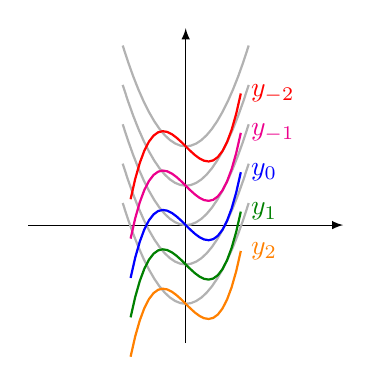
\begin{tikzpicture}[>=latex, scale=0.5]
				\draw [->] (-4,0) -- (4,0);
				\draw [->] (0,-3) -- (0,5);
				\foreach \n in {-2,...,2} \draw [thick , black!30, domain=-1.6:1.6] plot(\x , {pow(\x,2) +\n});
				\draw [thick ,red, domain=-1.4:1.4]     plot(\x , {pow(\x,3)-\x+2}) node [right] {\(y_{-2}\)};
				\draw [thick ,magenta, domain=-1.4:1.4] plot(\x , {pow(\x,3)-\x+1}) node [right] {\(y_{-1}\)};
				\draw [thick ,blue, domain=-1.4:1.4]    plot(\x , {pow(\x,3)-\x  }) node [right] {\(y_0\)};
				\draw [thick ,green!50!black, domain=-1.4:1.4]   plot(\x , {pow(\x,3)-\x-1}) node [right] {\(y_1\)};
				\draw [thick ,orange, domain=-1.4:1.4]  plot(\x , {pow(\x,3)-\x-2}) node [right] {\(y_2\)};
			\end{tikzpicture}
		\end{columns}
	\end{example}
\end{frame}

\begin{frame}[t]
	\vspace{-3mm}
	\begin{exampleblock}{}
		La solución que pasa por \((0,1)\) tiende a \(\infty\) cuando \(x \longrightarrow \infty\), y tiende a \(- \infty\) cuando \(x \longrightarrow - \infty\).
	\end{exampleblock}
	\vspace{-2mm}
	\begin{example}
		\small
		Trace el campo direccional de la E.D. \(\frac{dy}{dx} -y^2=x^2\). Y bosqueje las curvas solución. \\
		\textbf{Solución.} La E.D. en forma normal es \(\dfrac{dy}{dx} =x^2+y^2\).
		\vspace{-4mm}
		\begin{columns}
			\column{0.4\textwidth}
			\[
				x^2+y^2=c.
			\]
			\begin{tabular}{r|l}
				\(c\) & Isoclina \\ \hline
				\(0\) & \(I_0=x^2+y^2=0\) \\
				\(1\) & \(I_1=x^2+y^2=1\) \\
				\(2\) & \(I_1=x^2+y^2=2\) \\
				\(4\) & \(I_4=x^2+y^2=4\)
			\end{tabular}\\
			Note que \(\dfrac{dy}{dx} =x^2+y^2 \geqslant 0\),
			\column{0.5\textwidth}
			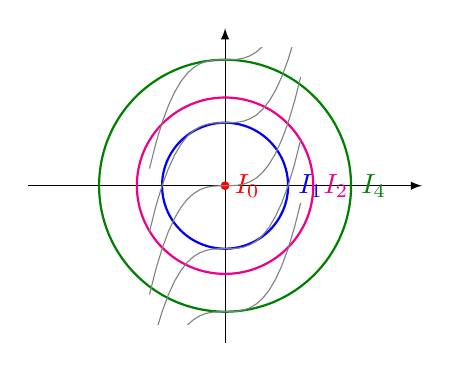
\begin{tikzpicture}[>=latex]
				\draw [->] (-2.5,0) -- (2.5,0);
				\draw [->] (0,-2) -- (0,2);
				\begin{scope}[scale=0.8]
					\fill [red] (0,0) circle (2pt) node [right] {\(I_0\)};
					\draw [thick, blue] (0,0) circle (1cm) node [right=8mm] {\(I_1\)};
					\draw [thick, magenta] (0,0) circle (1.4cm) node [right=1.12cm] {\(I_2\)};
					\draw [thick, green!50!black] (0,0) circle (2cm) node [right=1.6cm] {\(I_4\)};
					\clip (-2.2,-2.2) rectangle (2.2,2.2);
					\foreach \n in {-2,...,2} \draw [gray, domain=-1.2:1.2] plot(\x , {pow(\x,3)+\n});
				\end{scope}
			\end{tikzpicture}
		\end{columns}
		\(\forall (x,y) \in \mathbb{R} ^2\). Por lo tanto, todas las soluciones \(y(x)\) de la E.D. son crecientes \(\forall x \in \mathbb{R}\).
	\end{example}
\end{frame}

% )))

% )))

\section{6. Análisis Cualitativo para E.D. Autónomas.} % (((

\begin{frame}[t]
	\frametitle{6. Análisis Cualitativo para E.D. Autónomas.}
	\vspace{-2mm}
	\begin{definition}
		Se dice que una E.D. de Primer Orden es una ecuación diferencial \textbf{autónoma} si tiene la forma \(y\,' =f(y)\), donde \(f\) es una función de valor real (\(f: \Omega \longrightarrow \mathbb{R}\)), esto es, independiente de \(x\).
	\end{definition}
	\vspace{-2mm}
	\begin{example}
		Veamos si las sig. E.D. son autónomas.
		\begin{enumerate}
			\item \(\dfrac{dA}{dt} = kA\), con \(A=A(t)\). \textbf{(Desintegración Radioactiva)}.\\
				\textbf{Solución.} \(k\) es constante. E.D. autónoma.
			\item \(\dot{x} =k(x) (n+1-x)\), con \(x=x(t)\), \(k,n \in \mathbb{R}\). \textbf{(Poblaciones).}\\
				\textbf{Solución.} E.D. autónoma.
			\item \(\dfrac{dN}{dt} = 6t - \dfrac{N}{100}\). \textbf{(Mezclas)}.\\
				\textbf{Solución.} E.D. no autónoma.
		\end{enumerate}
	\end{example}
\end{frame}

\begin{frame}[t]
	\begin{exampleblock}{}
		\begin{enumerate}
				\setcounter{enumi}{3}
			\item \(\dfrac{dT}{dt} =k(T-T_n)\). \textbf{(Ley de Enfriamiento de Newton).}\\
				\textbf{Solución.} \(T=T(t)\), \(k,T_n \in \mathbb{R}\), E.D. autónoma.
		\end{enumerate}
	\end{exampleblock}
	El bosquejo del cambio de dirección de una E.D. de la forma \(y\,' =f(y)\), autónoma, es particularmente sencillo, dado que \(f\) es independiente de \(x\). Por lo cual, las pendientes son idénticas a lo largo de rectas (ecuaciones) horizontales.
	\begin{example}
		\small 
		Considere la E.D. \(y\,'=y\). Usemos el método de las isoclinas para esbozar su gráfica de las soluciones de la E.D.
		\begin{columns}
			\column{0.3\textwidth}
			\(y\,' =y\).\\
			\begin{tabular}{r|l}
				\(c\) & Isoclinas \\ \hline
				\(1\) & \(y_{-1} =-1\) \\
				\(0\) & \(y_0=0\) \\
				\(1\) & \(y_1=1\)
			\end{tabular}
			\column{0.6\textwidth}
			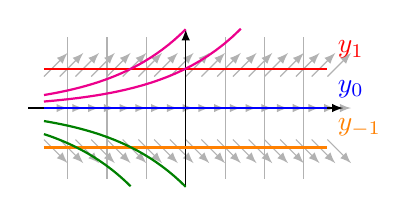
\begin{tikzpicture}[>=latex]
				\foreach \n in {-1.5,-1,...,1.5} \draw [black!30] (\n,-0.9) --++ (0,1.8);
				\foreach \n in {-1.8,-1.6,...,1.8} \draw [black!30,->] (\n,0.4) --++ (0.3,0.3);
				\foreach \n in {-1.8,-1.6,...,1.8} \draw [black!30,->] (\n,0) --++ (0.3,0);
				\foreach \n in {-1.8,-1.6,...,1.8} \draw [black!30,->] (\n,-0.4) --++ (0.3,-0.3);
				\draw [->] (-2,0) -- (2,0);
				\draw [->] (0,-1) -- (0,1);
				\draw [thick,red]    (-1.8,0.5)  --++ (3.6,0) node [above right] {\(y_1\)};
				\draw [thick,blue]   (-1.8,0)    --++ (3.6,0) node [above right] {\(y_0\)};
				\draw [thick,orange] (-1.8,-0.5) --++ (3.6,0) node [above right] {\(y_{-1}\)};
				\draw [thick , magenta, domain=-1.8:0.7] plot(\x , {0.5*exp(\x)});
				\draw [thick , magenta, domain=-1.8:0] plot(\x , {exp(\x)});
				\draw [thick , green!50!black, domain=-1.8:0] plot(\x , {-exp(\x)});
				\draw [thick , green!50!black, domain=-1.8:-0.7] plot(\x , {-2*exp(\x)});
			\end{tikzpicture}
		\end{columns}
	\end{example}
\end{frame}

\begin{frame}[t]
	\vspace{-4mm}
	\begin{definition}
		Se dice que \(a \in \mathbb{R}\) es un \textbf{punto de equilibrio} de una ecuación diferencial autónoma \(y\,' =f(y)\) si \(a\) es un cero o raíz de \(f\). A un punto de equilibrio también se le conoce como \textbf{punto estacionario}, \textbf{punto fijo}, o \textbf{punto crítico}. 
	\end{definition}
	Todo punto de equilibrio \(a\) define una solución constante de la E.D. autónoma.
	\[
		y(x) \equiv a, \hspace{5mm} \forall x \in \mathbb{R} .
	\]
	a tal solución se le conoce como \textbf{solución de equilibrio} o \textbf{estacionaria}. Veamoslo.\\
	Sea \(a \in \mathbb{R}\), un punto de equilibrio de E.D. \(f(a) =0\).\\
	Luego, sea \(y(x) \equiv a\), veamos si es solución de la E.D.
	\[
		\begin{array}{rcl}
			y\,' & = & f(y) \\[2mm]
			0 = (a) ' & = & f(a) =0
		\end{array}
	\]
\end{frame}

\begin{frame}[t]
	\vspace{-2mm}
	Para las E.D. autónomas su interpretación geométrica queda determinada por \(f(y)\). Así pues, averigüar cómo es la pendiente sobre el eje \(y\) a partir de la gráfica de \(f\), es de gran utilidad para esbozar las soluciones de la ecuación diferencial y obtener información acerca de su comprtamiento.\\
	Para ilustrar lo anterior, consideremos una E.D. \(y\,' =f(y) \) donde la gráfica de \(f\) tiene la siguiente forma.
	\vspace{-2mm}
	\begin{columns}
		\column{0.5\textwidth}
		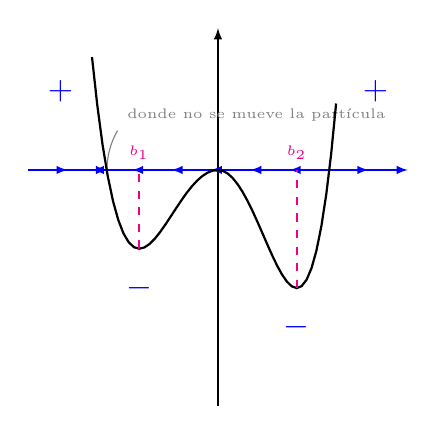
\begin{tikzpicture}[>=latex]
			\draw [->] (0,-3) -- (0,1.8);
			\begin{scope}[blue,->]
				\foreach \n in {1,2} \draw (1.41,0) --++ (\n*0.5,0);
				\foreach \n in {1,...,6} \draw (1.41,0) --++ (-\n*0.5,0);
				\foreach \n in {1,2} \draw (-2.41,0) --++ (\n*0.5,0);
			\end{scope}
			\draw [gray] (-1.41,0) arc (180:150: 1 cm) node [above right] {\tiny donde no se mueve la partícula};
			\draw [thick , domain=-1.6:0] plot(\x , {pow(\x,4) -2*pow(\x,2)});
			\draw [thick , domain=0:1.5] plot(\x , {1.5*pow(\x,4) -3*pow(\x,2)});
			\draw [dashed , magenta, thick] (-1,-1) --++ (0,1) node [above] {\tiny \(b_1\)};
			\draw [dashed , magenta , thick] (1,-1.5) --++ (0,1.5) node [above] {\tiny \(b_2\)};
			\estabilidad{-1.41,0}{\CIRCLE}{pozo}{below left}{green!70!black}
			\estabilidad{0,0}{\LEFTcircle}{silla}{below left}{green!70!black}
			\estabilidad{1.41,0}{\Circle}{fuente}{below right}{green!70!black}
			\node[blue] at (2,1) {\large \(+\)};
			\node[blue] at (-2,1) {\large \(+\)};
			\node[blue] at (1,-2) {\large \(-\)};
			\node[blue] at (-1,-1.5) {\large \(-\)};
		\end{tikzpicture}
		\column{0.5\textwidth}
		Imaginemos que \(y=y(x)\) es la posición de una partícula que se mueve a lo largo de una línea recta con el tiempo. \\[2mm]
		La gráfica de \(f\) proporciona información sobre la característica de monotonía y concavidad de las soluciones \(y=y(x)\).
	\end{columns}
\end{frame}

\begin{frame}[t]
	\vspace{-4mm}
	\begin{block}{Monotonía}
		\begin{enumerate}
			\item Si \(y\,' =f(y) >0\) entonces \(y(x)\) es creciente.
			\item Si \(y\,' =f(y) <0\) entonces \(y(x)\) es decreciente.
		\end{enumerate}
	\end{block}
	\vspace{-2mm}
	\begin{block}{Concavidad}
		\begin{enumerate}
			\item \(y\,'' =f\,' (y) \cdot y\,' >0\) entonces \(y(x)\) es convexa (cóncava hacia arriba).
			\item \(y\,'' =f\,' (y) \cdot y\,' <0\) entonces \(y(x)\) es cóncava (cóncava hacia abajo).
		\end{enumerate}
	\end{block}
	\vspace{-2mm}
	También es posible encontrar puntos de inflexión.
	\[
		\begin{array}{rcl}
			y \;:\; y\,'' = f\,'(y) \cdot y\,' =0. && f\,' (y) \cdot f(y) =0. \\[2mm]
			\iff f\,' (y) =0 & \mbox{o} & y\,' =f(y) =0. \\[2mm]
			\mbox{Pts. Inflexión} && \mbox{Pts. de Equilibrio}
		\end{array}
	\]
	Para este ejemplo, los puntos de inflexión son \(y_1=b_1 \;,\; y_2=b_2\) para soluciones.
\end{frame}

\begin{frame}[t]
	\vspace{-3mm}\small
	\begin{figure}[ht]
		\centering
		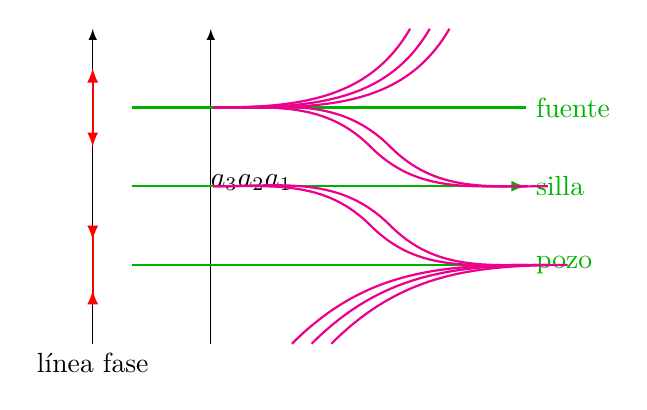
\begin{tikzpicture}[>=latex]
			\draw [->] (0,-2) -- (0,2);
			\draw [green!70!black, thick ,->] (-1,0) -- (4,0) node [right] {silla};
			\def\rad{0.5}
			\draw [->] (-1.5,-2) node [below] {línea fase} --++ (0,4);
			\draw [thick,<-> , red] (-1.5,1-\rad) -- (-1.5,1+\rad);
			\draw [thick,>-<, red] (-1.5,-1-\rad) -- (-1.5,-1+\rad);
			\draw [thick ,green!70!black] (-1,1) --++ (5,0) node [right] {fuente} (-1,-1) --++ (5,0) node [right] {pozo};
			\estabilidad{-1.5,1}{\Circle}{\(a_3\)}{left}{red}
			\estabilidad{-1.5,0}{\LEFTcircle}{\(a_2\)}{left}{red}
			\estabilidad{-1.5,-1}{\CIRCLE}{\(a_1\)}{left}{red}
			\draw [thick , magenta] (-1,1) to [out=0 , in=240] (1.5,2); 
			\draw [thick , magenta] (-1,1) to [out=0 , in=240] (1.75,2); 
			\draw [thick , magenta] (-1,1) to [out=0 , in=240] (2,2); 
			\draw [thick , magenta] (-1,1) to [out=0 , in=135] (1,0.5) to [out=-45,in=180] (3,0);
			\draw [thick , magenta] (-1,1) to [out=0 , in=135] (1.25,0.5) to [out=-45,in=180] (3.25,0);
			\draw [thick , magenta] (-1,0) to [out=0 , in=135] (1,-0.5) to [out=-45,in=180] (3,-1);
			\draw [thick , magenta] (-1,0) to [out=0 , in=135] (1.25,-0.5) to [out=-45,in=180] (3.25,-1);
			\draw [thick , magenta] (0,-2)to [out=45 , in=-180] (3,-1); 
			\draw [thick , magenta] (0.25,-2)to [out=45 , in=-180] (3.25,-1); 
			\draw [thick , magenta] (0.5,-2)to [out=45 , in=-180] (3.5,-1); 
		\end{tikzpicture}
	\end{figure}
	\tiny
		\begin{tabular}{ccccll}
			\color{blue} Intervalos de \(y\) &\color{blue} Signo de &\color{blue} Pts. Inflexión &\color{blue} Subintervalos &\color{blue} Signo \(y''\) &\color{blue} Características \(y\) \\
			& \color{blue} \(y\,' =f(y)\) &&&&\\
			\((- \infty , a_1)\) & \((+)\) & --- & --- & \(y'' = (+) (-) =(-)\) & Creciente, cóncava.\\
			\((a_1,a_2)\) & \((-)\) & \(y_1=b\) & \((a_1,b_1)\) & \(y'' = (-) (-) =(+)\) & Decreciente, convexa \\
			& & & \((b_1,b_2)\) & \(y'' = (-) (+) = (-)\) & Decreciente, cóncava\\
			\((a_2,a_3)\) & \((-)\) & \(y_2 =b_2\) & \((a_2,b_3)\) & \(y'' = (-) (-) = (+)\) & Decreciente, convexa \\
			&&& \((b_2,a_3)\) & \(y'' = (-) (+) = (-)\) & Decreciente, cóncava \\
			\((a_3, \infty)\) & \((+)\) & --- & --- & \(y'' =(+) (+) =(+)\) & Creciente, convexa
		\end{tabular}
\end{frame}

\begin{frame}[t]
	\begin{definition}
		\begin{enumerate}
			\item Un punto de equilibrio se dice que un \textbf{pozo} o \textbf{sumidero} cuando el flujo local a su alrededor del punto se dirige hacia él.
			\item Un punto de equilibrio se dice que es una \textbf{fuente} cuando el flujo local alrededor del punto se aleja de él.
			\item Y un punto de equilibrio se dice \textbf{silla} o \textbf{nodo} cuando el flujo local por un lado se dirige hacia él, y por el otro lado se aleja,
		\end{enumerate}
	\end{definition}
	\begin{definition}
		Al punto de equilibrio pozo o sumidero, se le conoce como \textbf{punto de equilibrio estable}, a la fuente como \textbf{punto de equilibrio inestable} y a los puntos silla como \textbf{semiestables}.
	\end{definition}
\end{frame}

\begin{frame}[t]
	\vspace{-4mm}
	\begin{definition}
		El \textbf{retrato fase} es el conjunto de todas las soluciones y se acostumbra a representarlo con una recta real, donde las flechas representan al campo vectorial y los puntos corresponden a los puntos de equilibrio y su estabilidad. \\[2mm]
		También se le conoce como \textbf{línea fase} o \textbf{retrato fase unidimensional}.
	\end{definition}
	\vspace{-2mm}
	\begin{example}
		Considere la E.D. autónoma \(y' -y^3+2y^2-y=0\).
		\begin{enumerate}
			\item Determine las soluciones de equilibrio y utilice la línea fase para clasificarlas como pozos, fuentes o sillas.
			\item Esboza algunas curvas solución de la E.D. incluyendo las soluciones de equilibrio.
			\item Indica el comportamiento de la solución que satisface la condición inicial \(y(0) =1/2\), cuando \(t \longrightarrow \infty\).
		\end{enumerate}
	\end{example}
\end{frame}

\begin{frame}[t]
	\begin{exampleblock}{}
		\textbf{Solución.} 
		\begin{enumerate}
			\item La forma normal de la E.D. es
				\[
					y\,' = y^3-2y^2+y = y(y^2-2y+1) = y(y-1) ^2=f(y).
				\]
				Encontremos \(y\) tal que \(f(y) =0\), es decir
				\[
					\begin{array}{rcl}
						y(y-1) ^2 & = & 0 \\[2mm]
						\iff y_1=0 & \mbox{ó} & (y-1) ^2=0. \\[2mm]
						\iff && y_2=1.
					\end{array}
				\]
				\(\therefore \hspace{3mm}\) se tienen 2 puntos.\\
				Luego, las soluciones de equilibrio son \(y_1(x) =0\) y \(y_2(x) =1\).
		\end{enumerate}
	\end{exampleblock}
\end{frame}

\begin{frame}[t]
	\begin{exampleblock}{}
		Grafiquemos \(f(y)\), para determinar la línea fase.
		\begin{columns}
			\column{0.4 \textwidth}
			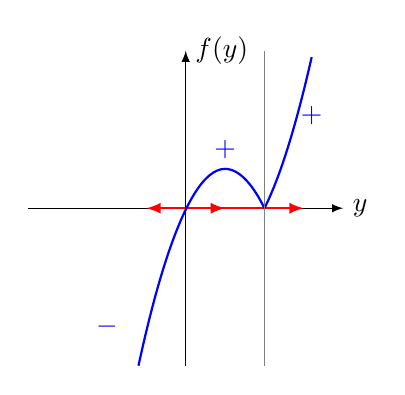
\begin{tikzpicture}[>=latex]
				\draw [->] (-2,0) -- (2,0) node [right] {\(y\)};
				\draw [->] (0,-2) -- (0,2) node [right] {\(f(y)\)};
				\draw [thick ,red,->] (0,0) -- (-0.5,0);
				\draw [thick , red,->] (0,0) -- (0.5,0);
				\draw [thick ,red,->] (0,0) -- (1.5,0);
				\draw [blue , thick] (-0.6,-2) parabola bend (0.5,0.5) (1,0);
				\draw [thick , blue, domain=1:1.6] plot(\x , {2*pow(\x-0.5,2) -0.5}) node [below=5mm] {\(+\)};
				\draw [gray] (1,-2) -- (1,2);
				\estabilidad{0,0}{\Circle}{fuente} {above left}{blue}
				\estabilidad{1,0}{\LEFTcircle}{silla}{below right}{blue}
				\node [blue, above] at (0.5,0.5) {\(+\)};
				\node [blue] at (-1,-1.5) {\(-\)};
			\end{tikzpicture}
			\column{0.5\textwidth}
			Por lo tanto \(y_1=0\) es fuente, y \(y_2=1\) es silla. \\[2mm]
			Los puntos de inflexión son los \(y\) tal que \(f(y) =0\), pero no son puntos de equilibrio. Derivemos.
			\[
				\begin{array}{rcl}
					f\,' (y) & = & 3y^2-4y+1 \\[2mm]
					& = & (3y-1) (y-1) =0 \\[2mm]
				\end{array}
			\]
		\end{columns}
		\[
			\begin{array}{rcl}
				\iff 3y-1=0 & \mbox{ó} & y-1=0 \\[2mm]
				\iff y_1= \dfrac{1}{3} && y_2=1 \\[2mm]
				\mbox{pto. inflexión} && \mbox{pto. de equlibrio}
			\end{array}
		\]
	\end{exampleblock}
\end{frame}

\begin{frame}[t]
	\begin{exampleblock}{}
	\begin{columns}
		\column{0.4\textwidth}
		\begin{enumerate}
				\setcounter{enumi}{1}
			\item
				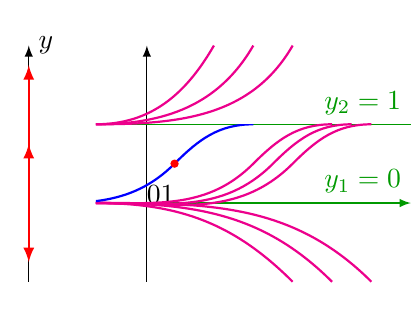
\begin{tikzpicture}[>=latex]
					\draw [->] (0,-1) -- (0,2);
					\draw [->] (-1.5,-1) --++ (0,3) node [right] {\(y\)};
					\draw [thick , red,<->] (-1.5,-0.75) --++ (0,1.5);
					\draw [thick ,red,->] (-1.5,0) --++ (0,1.75);
					\estabilidad{-1.5,0}{\Circle}{\(0\)}{left}{red}
					\estabilidad{-1.5,1}{\LEFTcircle}{\(1\)}{left}{red}
					\draw [green!60!black,->] (-1,0) -- (3,0) node [above left] {\(y_1=0\)};
					\draw [green!60!black] (-1,1) --++ (4,0) node [above left] {\(y_2=1\)};
					\draw [thick , magenta] (-1,1) to [out=0 , in=240] (0.5,2); 
					\draw [thick , magenta] (-1,1) to [out=0 , in=240] (1,2); 
					\draw [thick , magenta] (-1,1) to [out=0 , in=240] (1.5,2); 
					\draw [thick , magenta] (-1,0) to [out=0 , in=225] (1,0.5) to [out=45,in=180] (2,1); 
					\draw [thick , magenta] (-1,0) to [out=0 , in=225] (1.25,0.5) to [out=45,in=180] (2.25,1); 
					\draw [thick , magenta] (-1,0) to [out=0 , in=225] (1.5,0.5) to [out=45,in=180] (2.5,1); 
					\draw [thick , magenta] (-1,0) to [out=0 , in=135] (1.5,-1); 
					\draw [thick , magenta] (-1,0) to [out=0 , in=135] (2,-1); 
					\draw [thick , magenta] (-1,0) to [out=0 , in=135] (2.5,-1); 
					\clip (-1,0) rectangle (3,1);
					\draw [thick , blue] (-2,0) to [out=0 , in=225] (0,0.5) to [out=45,in=180] (1,1); 
					\fill [red] (0,0.5) circle (1.5pt);
				\end{tikzpicture}
		\end{enumerate}
		\column{0.5\textwidth}
		\begin{enumerate}
				\setcounter{enumi}{2}
			\item La {\color{blue}solución} que pasa por \(\color{red}(0,1/2)\) tiende a la recta \(y=1\) cuando \(t \longrightarrow \infty\),
		\end{enumerate}
	\end{columns}
	\tiny 
		\begin{tabular}{*{6}{l}}
			\color{blue} Intervalos &\color{blue} Signo de &\color{blue} P.I. &\color{blue} Subintervalos &\color{blue} Signo \(y\,''\) &\color{blue} Características \(y(t)\) \\
			& \color{blue} \(y\,' =f(y)\) & &&&\\
			\((- \infty ,0)\) & \((-)\) & --- & \((- \infty ,0)\) & \((-) (+) =(-)\) & Decreciente, cóncava\\
			\((0,1)\) & \((+)\) & \(y_1=1/3\) & \((0,1/3)\) & \((+) (+) =(+)\) & Creciente, convexa \\
			& & --- & \((1/3,1)\) & \((+) (-) =(-)\) & Creciente, cóncava\\
			\((1, \infty)\) & \((+)\) & --- & \((1, \infty)\) & \((+) (+) =(+)\) & Creciente, convexa
		\end{tabular}
	\end{exampleblock}
\end{frame}

\begin{frame}[t]
	\vspace{-4mm}
	\begin{example}
		Considere la E.D. \(y\,' =-(y-1) ^{5/3} (y-2) ^2(y-3)\). Encuentre la solución de equilibrio de la ecuación diferencial y clasifíquelos usando la línea fase. Esboce algunas soluciones incluyendo las soluciones de equilibrio, considerando su característica de monotonía y concavidad. Por último, predecir el comportamiento que tiene la solución que satisface \(y(0) =2.1\) cuando \(t \longrightarrow \infty\). \\[2mm]
		\textbf{Solución.} La forma normal de la E.D. es
		\[
			y\,' = -(y-1) ^{5/3} (y-2) ^2(y-3) =f(y).
		\]
		Encontremos \(y\) tal que \(f(y) =0\), es decir
		\[
			\begin{array}{rcl}
				-(y-1) ^{5/3} (y-2) ^2(y-3) & = & 0 \\[2mm]
				\iff (y-1) ^{5/3} =0 \hspace{2mm} \mbox{ó} \hspace{2mm} (y-2) ^2 & = & 0 \hspace{2mm} \mbox{ó} \hspace{2mm} y-3=0 \\
				\iff y_1=1 \hspace{1.5cm} \mbox{ó} \hspace{4mm} y_2=2 && \hspace{3mm} \mbox{ó} \hspace{2mm} y_3=3.
			\end{array}
		\]
	\end{example}
\end{frame}

\begin{frame}[t]
	\begin{exampleblock}{}
		\(\therefore \hspace{3mm}\) se tienen \(3\) puntos de equilibrio. \\[2mm]
		Luego, las soluciones de equilibrio son 
		\[
			y(x) =1 \;,\; y(x) =2 \;,\; y_3(x) =3.
		\]
		grafiquemos para determinar la línea fase. \vspace{-3mm}
		\begin{figure}[ht]
			\centering
			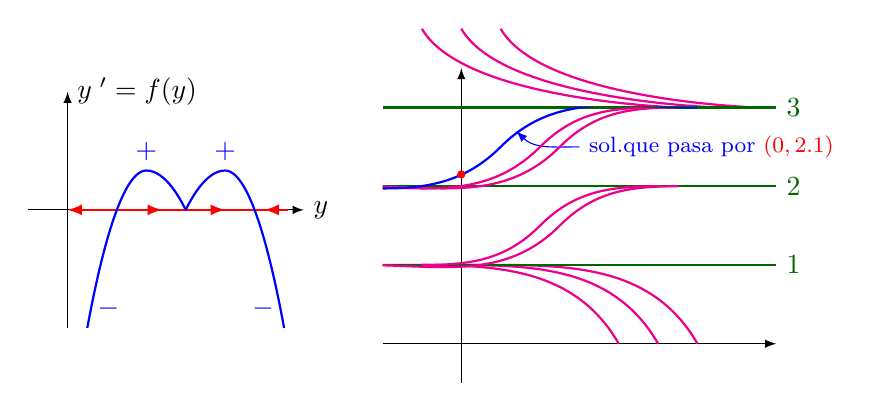
\begin{tikzpicture}[>=latex]
				\draw [->] (-1,0) -- (2.5,0) node [right] {\(y\)};
				\draw [thick ,red,<->] (-0.5,0) -- (0.7,0);
				\draw [thick ,red,->] (0.5,0) -- (1.5,0);
				\draw [thick ,red] (1.3,0) -- (2.3,0);
				\draw [thick ,red,->] (2.3,0) -- (2,0);
				\draw [->] (-0.5,-1.5) -- (-0.5,1.5) node [right] {\(y\;' =f(y)\)};
				\draw [thick , blue] (-0.25,-1.5) node [above right] {\(-\)} parabola bend (0.5,0.5) (1,0);
				\draw [thick , blue] (1,0) parabola bend (1.5,0.5) (2.25,-1.5) node [above left] {\(-\)};
				\node [blue , above] at (0.5,0.5) {\(+\)};
				\node [blue , above] at (1.5,0.5) {\(+\)};
				\estabilidad{0.13,0}{\Circle}{fuente}{below right}{blue}
				\estabilidad{1,0}{\LEFTcircle}{silla}{below right}{blue}
				\estabilidad{1.87,0}{\CIRCLE}{pozo}{above right}{blue}
				\begin{scope}[shift={(4.5,0.3)}]
					\draw [->] (0,-2.5) -- (0,1.5);
					\draw [->] (-1,-2) --++ (5,0);
					\draw [thick , magenta] (-0.5,2) to [out=-60, in=0] (2.5,1); 
					\draw [thick , magenta] (0,2) to [out=-60, in=0] (3,1); 
					\draw [thick , magenta] (0.5,2) to [out=-60, in=0] (3.5,1); 
					\draw [thick , magenta] (-1,-1) to [out=0 , in=120] (2,-2); 
					\draw [thick , magenta] (-0.5,-1) to [out=0 , in=120] (2.5,-2); 
					\draw [thick , magenta] (0,-1) to [out=0 , in=120] (3,-2); 
					\draw [thick , green!40!black] (-1,1)  --++ (5,0) node [right] {\(3\)};
					\draw [thick , green!40!black] (-1,0)  --++ (5,0) node [right] {\(2\)};
					\draw [thick , green!40!black] (-1,-1) --++ (5,0) node [right] {\(1\)};
					\estabilidad{0,1}{\CIRCLE}{}{above}{green!60!black}
					\draw [blue,->] (1.5,0.5) node [right] {\footnotesize sol.que pasa por \(\color{red} (0,2.1)\)} to [out=180 , in=-45] (0.7,0.7);
					\clip (-1,-2) rectangle (3,1);
					\draw [thick , magenta] (-1.5,0) to [out=0 , in=225] (1,0.5) to [out=45,in=180] (2.5,1);
					\draw [thick , magenta] (-1.25,0) to [out=0 , in=225] (1.25,0.5) to [out=45,in=180] (2.75,1);
					\draw [thick , magenta] (-0.5,-1) to [out=0 , in=225] (1,-0.5) to [out=45,in=180] (2.5,0);
					\draw [thick , magenta] (-1.25,-1) to [out=0 , in=225] (1.25,-0.5) to [out=45,in=180] (2.75,0);
					\estabilidad{0,0}{\LEFTcircle}{}{above}{green!60!black}
					\estabilidad{0,-1}{\Circle}{}{above}{green!60!black}
					\draw [thick ,blue] (-2,0) to [out=0 , in=225] ++(2.5,0.5) to [out=45,in=180] ++(2.5,0.5); 
					\fill [red] (0,0.15) circle (1.5pt);
				\end{scope}
			\end{tikzpicture}
		\end{figure}
	\end{exampleblock}
\end{frame}

\begin{frame}[t]
	\begin{exampleblock}{}
		\[
			\begin{array}{c}
				f\,' (y) = - \dfrac{2}{3} (y-2) (y-1) ^{2/3} (7y^2-29y+27) =0 \\[2mm]
				\tilde{y} _1=2 \;,\; \tilde{y} _2=1 \;,\; \tilde{y} _3 = 2.73 \;,\; \tilde{y} _4 = 1.41.
			\end{array}
		\]
		\tiny
		\begin{tabular}{*{6}{l}}
			\color{blue} Intervalos de \(y\) & \color{blue} Signo de & \color{blue} P.I. & \color{blue} Subintervalos & \color{blue} Signo de & \color{blue} Características \(y(x)\) \\
			& \color{blue} \(y\,' =f(y)\) &&&&\\
			\((- \infty ,1)\) & \((-)\)  & --- & \((- \infty ,1)\) & \((-) (+) =(-)\) & Decreciente, cóncava\\
			\((1,2)\) & \((+)\) & \(y_4=1.41\) & \((1,1.41)\) & \((+) (+) =(+)\) & Creciente, convexa\\
			&&& \((1.41,2)\) & \((+) (-) =(-)\) & Creciente, cóncava\\
			\((2,3)\) & \((+)\) & \(y_3=2.73\) & \((2,273)\) & \((+) (+) =(+)\) & Creciente, cóncava\\
			&&& \((2.73,3)\) & \((+) (-) =(-)\) & Creciente convexa\\
			\((3, \infty)\) & \((-)\) & --- & \((3, \infty)\) & \((-) (-) =(+)\) & Decreciente, convexa
		\end{tabular}\\[4mm]
		\normalsize
		La solución que pasa por \(\color{red} (0,2.1)\) tiende a la recta \(y=3\), cuando \(t \longrightarrow \infty\).
	\end{exampleblock}
\end{frame}

\begin{frame}[t]
	\begin{alertblock}{Ejercicio}
		Considere la E.D. \(\dfrac{y\,'}{y+2} ) y^2-2y+ \frac 34\).
		\begin{enumerate}
			\item Determine los puntos de equilibrio de la E.D. autónoma y clasifícalos usando la línea fase.
			\item Indica cuál es el comportamiento de la solución de la E.D. que satisface la C.I. \(y(2/3) =1\), cuando \(x \longrightarrow \infty\), usando la línea fase.
			\item ¿Qué ocurre con la solución que pasa por \(y(1) =0\) cuando \(x \longrightarrow \infty\)? Usando la línea fase.
		\end{enumerate}
	\end{alertblock}
\end{frame}

% )))

\end{document}
